\chapter{Technology and method}
\lhead{\emph{Technology and method}}

In this chapter the technology and methods applied in this project are reasoned. The approach chosen will be explained in such a way that the results can be reconstructed.

\section{Technology}

\subsection{Version control}
In this project git has been used for the version control system through the hosting service Github. The reason for choosing Github was to be able to collaborate remotely and to always have a safe backup of the most recent version made.

\subsection{Collaboration tools}

In addition to using git for version control, ShareLaTeX and Office365 was also used for collaboration. 

ShareLaTeX is an online platform where multiple users can collaborate on the same LaTeX project in real time. LaTeX is a document preparation system for creating professional papers with great support for many document elements, such as equations and figures. Various packages can be used to further extend the functionality. 

Office 365 is available to all students at NTNU and offers cloud storage and emailing. The Office 365 platform enabled us to easily communicate with product owners and mentor in addition to storing project documents.


\subsection{Python and frameworks}
The choice of programming language was influenced mainly by its ability to integrate into already existing technology and the availability of machine learning tools. Python was a natural choice, as Matistikk is written in Django, a Python framework. In addition, Python was chosen due to its popular machine learning libraries TensorFlow and Keras. These libraries are closely connected, where Keras is used as an abstraction layer on top of TensorFlow. Keras was chosen to simplify the coding process and to be able to create quick prototypes.


A client application was also needed to draw symbols, collect data and present statistics. To keep the application architecture simple, HTML5, CSS and JavaScript with JQuery are used. In addition, the Python framework Tornado is used to serve the API and the client application. Tornado was chosen due to its simplicity and high performance.


\section{System Architecture}
The data used in this project is sequential coordinates from CROHME (InkML example: \ref{fig:InkML_ex}). Communication between the server and client application initially used WebSockets, both to resemble data format and to preserve information in sequential coordinates. For the sake of simplicity, it was also implemented a way to do this over a HTTP POST request. Several ways to handle web requests means that future developers can incorporate the software to fit their own needs.


\section{Preparing data}
This section will go through the process from when each symbol was segmented, to how the symbols were converted to input in the neural networks.

The data used as training data for the neural networks was in an XML format called InkML. In order to use this data as input to the neural networks, two main preprocessing steps were made. The data was first parsed, converted to NumPy arrays and normalized, then converted to images.

The data received from the front end application was processed in the same way, however, without parsing the InkML files. Opposed to the data received from InkML, this data was not already segmented, and the segmentation had to be completed first. The process for segmenting symbols is described in \ref{the_recognintion_system}.

The motivation for converting data to images was to use already existing models created for the MNIST dataset as a foundation for further work.

\subsection{Traces}
\label{preparing_data_traces}
The coordinates received from InkML and the front end application included coordinates at different scales. Therefore the coordinates had to be transformed within a chosen range $[-1, 1]$, while still keeping the same proportions. The scaling process is described in \ref{scale_linear_by_column}.

An example of a trace received from InkML can be seen in figure \ref{fig:sqrt_not_processed}.
\begin{figure}[H]
    \centering
    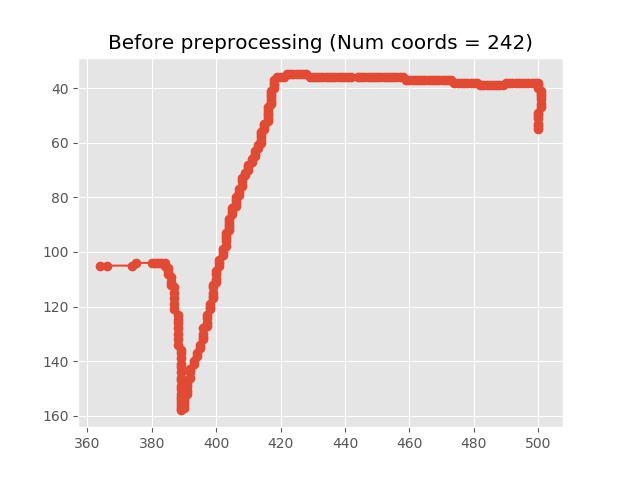
\includegraphics[width=\linewidth,keepaspectratio]{Assets/Chapter3_Method/sqrt_before_preprocessing.png}
    \caption{A square root as received from the InkML data.}
    \label{fig:sqrt_not_processed}
\end{figure}

The traces were recorded with different sampling frequencies. Some traces included several hundred points per symbol, while others included less than ten points per symbol. In order to improve performance of the networks, and make the input data normalized, the number of data points per symbol was reduced through a variant of the Ramer-Douglas-Peucker algorithm (\ref{ramer_douglas_peucker}). All symbols' data points were reduced to a maximum of 40 data points. If the original tracing had less than 40 data points, it was padded using leading zeros. An example of the resulting trace used as input to the RNN model can be seen below.

\begin{figure}[H]
    \centering
    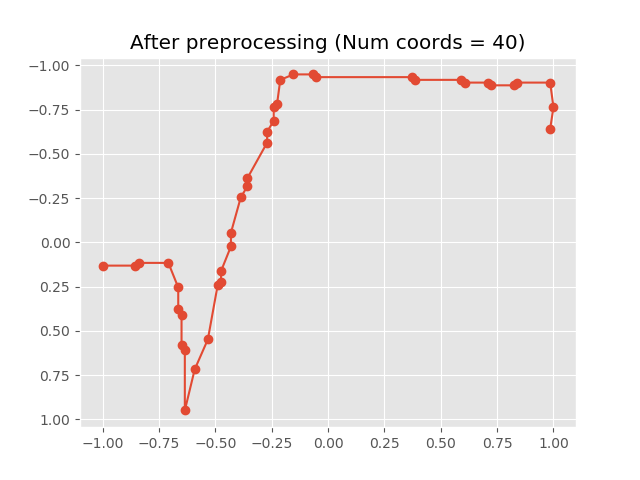
\includegraphics[width=\linewidth,keepaspectratio]{Assets/Chapter3_Method/sqrt_after_preprocessing.png}
    \caption{A square root after trace preprocessing.}
    \label{fig:sqrt_processed}
\end{figure}

\subsection{Images}

To prepare trace data for the convolutional neural network, the traces were converted into an image. First, the traces were scaled by applying the the same transformations as previously (\ref{scale_linear_by_column}), however within the range $[0, 26]$.

The next step was to generate an empty black image with 26x26 pixels (matrix of size 26x26 with only zeros). Afterwards, the pixels between each consecutive coordinate-pair were filled with white (255), and the resulting pixel grid was then normalized by dividing with 255. An example of the resulting grid presented as a matrix can be seen below, the example is simplified by using a 8x10 matrix.

\begin{figure}[H]
    \begin{center}
    $
    \begin{bmatrix} % Jobbe mer forklaringen, vi scaler ikke 26x26 til 4x4 (?)
        \textcolor{gray}{0} & \textcolor{gray}{0} & \textcolor{gray}{0} & \textcolor{gray}{0} & \textcolor{gray}{0} & \textcolor{gray}{0} & \textcolor{gray}{0} & \textcolor{gray}{0} & \textcolor{gray}{0} & \textcolor{gray}{0} \\
        \textcolor{gray}{0} & \textcolor{gray}{0} & \textcolor{gray}{0} & \textcolor{gray}{0} & 1 & 1 & 1 & 1 & 1 & \textcolor{gray}{0} \\
        \textcolor{gray}{0} & \textcolor{gray}{0} & \textcolor{gray}{0} & 1 & \textcolor{gray}{0} & \textcolor{gray}{0} & \textcolor{gray}{0} & \textcolor{gray}{0} & \textcolor{gray}{0} & 1 \\
        1 & \textcolor{gray}{0} & \textcolor{gray}{0} & 1 & \textcolor{gray}{0} & \textcolor{gray}{0} & \textcolor{gray}{0} & \textcolor{gray}{0} & \textcolor{gray}{0} & \textcolor{gray}{0} \\
        \textcolor{gray}{0} & 1 & \textcolor{gray}{0} & 1 & \textcolor{gray}{0} & \textcolor{gray}{0} & \textcolor{gray}{0} & \textcolor{gray}{0} & \textcolor{gray}{0} & \textcolor{gray}{0} \\
        \textcolor{gray}{0} & 1 & \textcolor{gray}{0} & 1 & \textcolor{gray}{0} & \textcolor{gray}{0} & \textcolor{gray}{0} & \textcolor{gray}{0} & \textcolor{gray}{0} & \textcolor{gray}{0} \\
        \textcolor{gray}{0} & 1 & \textcolor{gray}{0} & 1 & \textcolor{gray}{0} & \textcolor{gray}{0} & \textcolor{gray}{0} & \textcolor{gray}{0} & \textcolor{gray}{0} & \textcolor{gray}{0} \\
        \textcolor{gray}{0} & \textcolor{gray}{0} & 1 & \textcolor{gray}{0} & \textcolor{gray}{0} & \textcolor{gray}{0} & \textcolor{gray}{0} & \textcolor{gray}{0} & \textcolor{gray}{0} & \textcolor{gray}{0} \\

    \end{bmatrix}
    $
    \end{center}
    \caption{A 8x10 matrix representing a pixel grid of a square root symbol.} % burde nok ha litt mer forklaring, TODO flytt forklaringen ovenfor ned i caption. (?)
    \label{fig:sqrt_matrix}
\end{figure}

An image taken directly from the training data is visualized in figure \ref{fig:sqrt_img}. The resolution of the image is 26x26 pixels.

\begin{figure}[H]
    \centering
    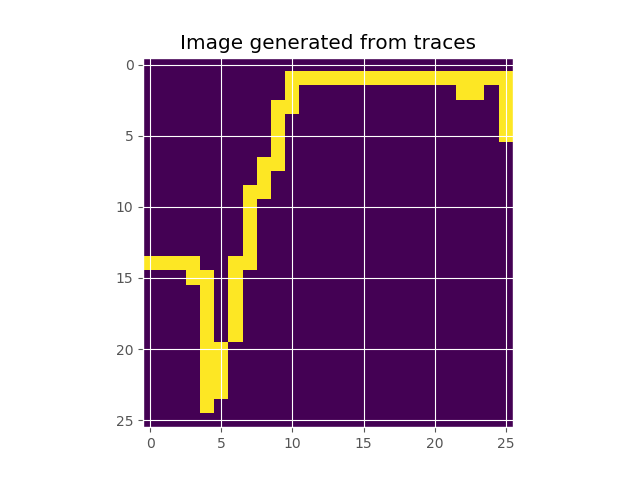
\includegraphics[width=\linewidth,keepaspectratio]{Assets/Chapter3_Method/sqrt_image.png}
    \caption{The resulting square root from the preprocessing done in previous steps.\\The generated image is 26x26 pixels.}
    \label{fig:sqrt_img}
\end{figure}

\section{The recognition system}
\label{the_recognintion_system}
The recognition system developed consists of several components, that together performs the common steps in handwriting recognition.

\subsection{Preprocessing and segmentation}
\label{preprocessing_and_segmentation}

The system begins with the segmentation, as the traces are sequential data and does not need to be preprocessed for the segmentation method chosen. The recognition system uses a simple approach for this, where traces that overlap are considered to be part of the same symbol. To find these groups, the coordinates of the traces are used to calculate distances and check for overlaps. If the distance between a coordinate in a trace to a coordinate in another trace is within a small threshold, the traces are grouped together.

After the traces are grouped, they are placed into a symbol object. Each of these symbol object receives a set of positional and proportional attributes based on the coordinates in the traces. Maximum and minimum values for both x- and y-coordinates are found, as well as width, height and the centre point. These attributes are used in the context search, described in section \ref{interpretation_context_search}. In addition, each symbol contains a truth value, which holds the classification results received in the next step.

Before the classification step the traces of each symbol are preprocessed as described in \ref{preparing_data_traces}. 

\subsection{Model architecture} 

The following section describes the architecture of three different models used in this project. A convolutional neural network, a recurrent neural network and a model combining both networks.

\subsubsection{RNN model}

The RNN model includes two one-dimensional convolution layers with max pooling and batch normalization. It also includes two bidirectional Gated Recurrent Unit layers. This model was first inspired by the Google Quick Draw model \cite{_recurrent_2017}. It has been modified to correspond with the train dataset's input- and output data. The model's architecture was also modified through experimentation, with the intention of producing better results on the test dataset. All models were compiled using the Adam optimizer and categorical cross entropy loss function \cite{chollet_keras_2015}.
\begin{figure}[H]
    \centering
    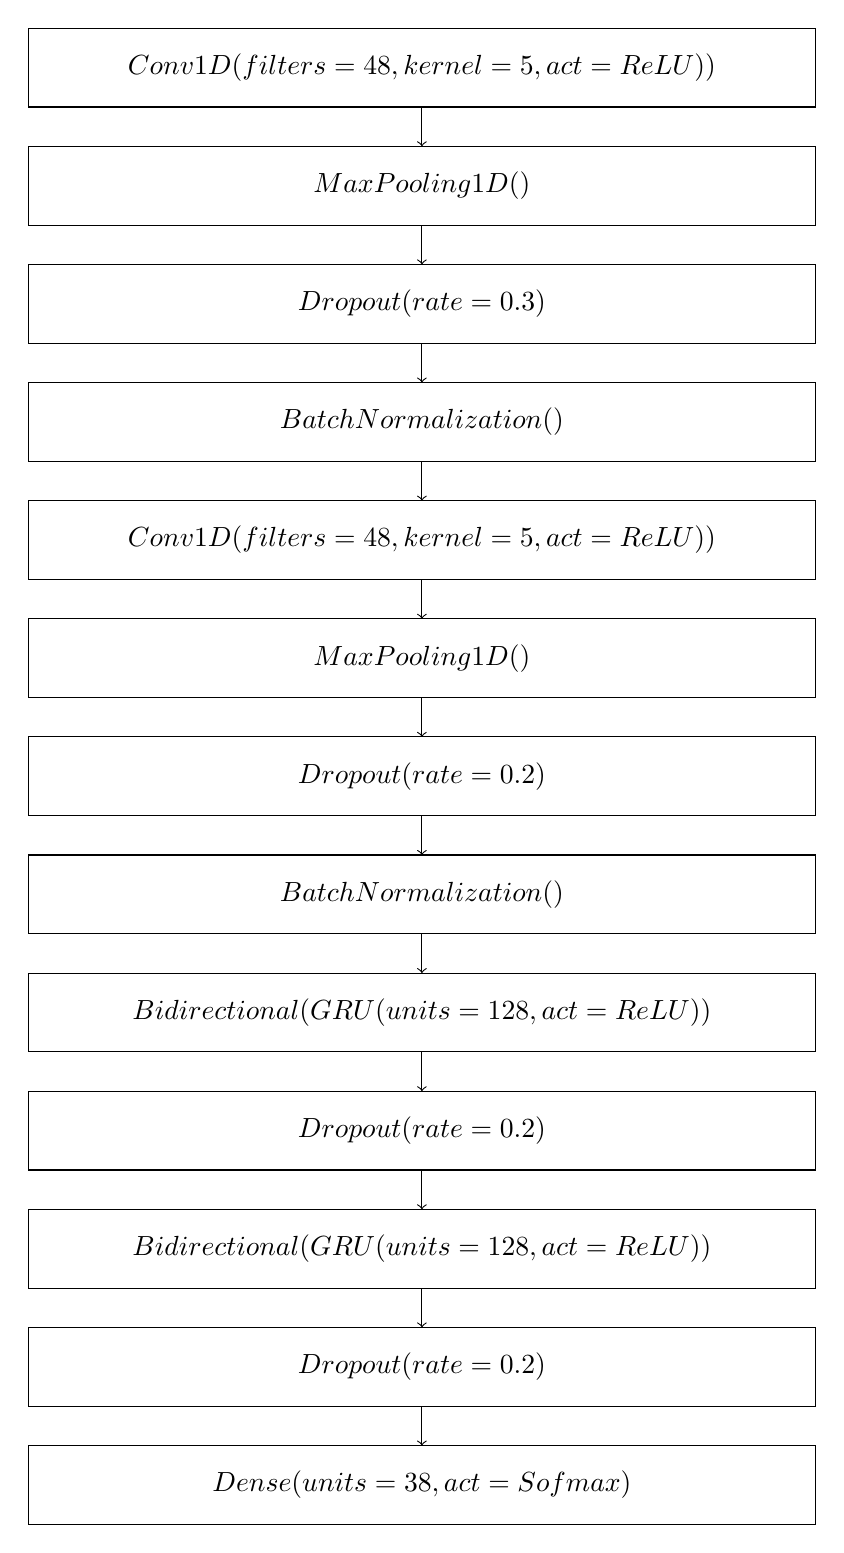
\begin{tikzpicture}
        \draw [black] (0, 1) rectangle (10, 0);
        \node[] at (5,0.5) {$Conv1D(filters=48, kernel=5, act=ReLU))$};
        \draw[->] (5, 0) -- (5, -0.5);
        
        \draw [black] (0, -0.5) rectangle (10, -1.5);
        \node[] at (5,0.-1) {$MaxPooling1D()$};
        \draw[->] (5, -1.5) -- (5, -2);

        \draw [black] (0, -2) rectangle (10, -3);
        \node[] at (5, -2.5) {$Dropout(rate=0.3)$};
        \draw[->] (5, -3) -- (5, -3.5);
        
        \draw [black] (0, -3.5) rectangle (10, -4.5);
        \node[] at (5, -4) {$BatchNormalization()$};
        \draw[->] (5, -4.5) -- (5, -5);
        
        \draw [black] (0, -5) rectangle (10, -6);
        \node[] at (5, -5.5) {$Conv1D(filters=48, kernel=5, act=ReLU))$};
        \draw[->] (5, -6) -- (5, -6.5);
        
        \draw [black] (0, -6.5) rectangle (10, -7.5);
        \node[] at (5, -7) {$MaxPooling1D()$};
        \draw[->] (5, -7.5) -- (5, -8);

        \draw [black] (0, -8) rectangle (10, -9);
        \node[] at (5, -8.5) {$Dropout(rate=0.2)$};
        \draw[->] (5, -9) -- (5, -9.5);
        
        \draw [black] (0, -9.5) rectangle (10, -10.5);
        \node[] at (5, -10) {$BatchNormalization()$};
        \draw[->] (5, -10.5) -- (5, -11);

        \draw [black] (0, -11) rectangle (10, -12);
        \node[] at (5, -11.5) {$Bidirectional(GRU(units=128, act=ReLU))$};
        \draw[->] (5, -12) -- (5, -12.5);

        \draw [black] (0, -12.5) rectangle (10, -13.5);
        \node[] at (5, -13) {$Dropout(rate=0.2)$};
        \draw[->] (5, -13.5) -- (5, -14);
        
        \draw [black] (0, -14) rectangle (10, -15);
        \node[] at (5, -14.5) {$Bidirectional(GRU(units=128, act=ReLU))$};
        \draw[->] (5, -15) -- (5, -15.5);
        
        \draw [black] (0, -15.5) rectangle (10, -16.5);
        \node[] at (5, -16) {$Dropout(rate=0.2)$};
        \draw[->] (5, -16.5) -- (5, -17);
        
        \draw [black] (0, -17) rectangle (10, -18);
        \node[] at (5, -17.5) {$Dense(units=38, act=Sofmax)$};


    \end{tikzpicture}
    \caption{A visualisation of the layer architecture in the RNN model. In depth description of each layer is available in the Keras documentation \cite{chollet_keras_2015}.}
    \label{fig:RNN__model_visualization_1}
\end{figure}

\subsubsection{CNN model}

The CNN model has two convolution layers, a max pooling layer and two fully connected layers. The model had issues with overfitting, and it therefore includes two dropout layers with  rate of 25\% and 50\% respectively. The model also includes a flatten layer. The flatten layer performs a dimensionality reduction on the matrix returned from the convolutional layers. This model is inspired by CNN models with good results on the MNIST dataset. \cite{ciresan_multi-column_2012}

\begin{figure}[H]
    \centering
    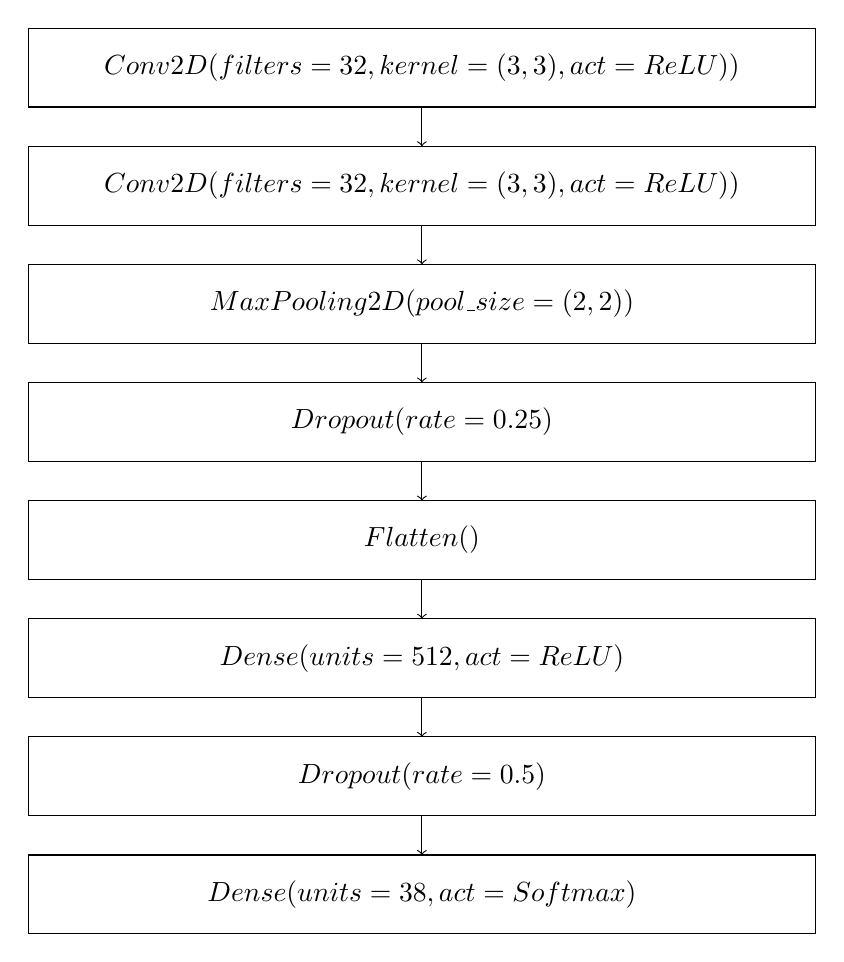
\begin{tikzpicture}
        \draw [black] (0, 1) rectangle (10, 0);
        \node[] at (5,0.5) {$Conv2D(filters=32, kernel=(3,3), act=ReLU))$};
        \draw[->] (5, 0) -- (5, -0.5);
        
        \draw [black] (0, -0.5) rectangle (10, -1.5);
        \node[] at (5,0.-1) {$Conv2D(filters=32, kernel=(3,3), act=ReLU))$};
        \draw[->] (5, -1.5) -- (5, -2);

        \draw [black] (0, -2) rectangle (10, -3);
        \node[] at (5, -2.5) {$MaxPooling2D(pool\_size=(2,2))$};
        \draw[->] (5, -3) -- (5, -3.5);
        
        \draw [black] (0, -3.5) rectangle (10, -4.5);
        \node[] at (5, -4) {$Dropout(rate=0.25)$};
        \draw[->] (5, -4.5) -- (5, -5);
        
        \draw [black] (0, -5) rectangle (10, -6);
        \node[] at (5, -5.5) {$Flatten()$};
        \draw[->] (5, -6) -- (5, -6.5);
        
        \draw [black] (0, -6.5) rectangle (10, -7.5);
        \node[] at (5, -7) {$Dense(units=512, act=ReLU)$};
        \draw[->] (5, -7.5) -- (5, -8);

        \draw [black] (0, -8) rectangle (10, -9);
        \node[] at (5, -8.5) {$Dropout(rate=0.5)$};
        \draw[->] (5, -9) -- (5, -9.5);
        
        \draw [black] (0, -9.5) rectangle (10, -10.5);
        \node[] at (5, -10) {$Dense(units=38, act=Softmax)$};

    \end{tikzpicture}
    \caption{A visualisation of the layer architecture in the CNN model. In depth description of each layer is available in the Keras documentation \cite{chollet_keras_2015}.}
    \label{fig:RNN__model_visualization_2}
\end{figure}

\subsubsection{Combined model}

The combined model's architecture is a concatenation of the results from both the CNN- and RNN model. The two model's last fully connected layer was removed before concatenation, to preserve as much information as possible. The combined model also has two fully connected layers and a dropout layer. The purpose of these layers is to enable the model to make its own predictions from the results of both input models.
\begin{figure}[H]
    \centering
    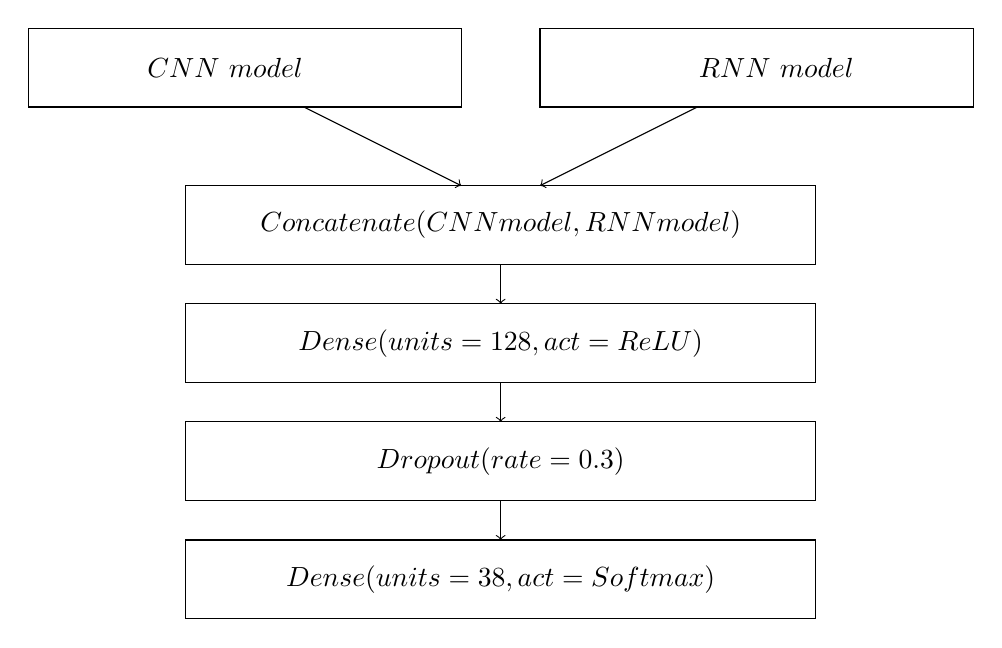
\begin{tikzpicture}
        \draw [black] (-6, -1) rectangle (-0.5, 0);
        \node[] at (-3.5,-0.5) {$CNN\ model$};
        \draw[[->] (-2.5, -1) -- (-0.5, -2);

        \draw [black] (0.5, -1) rectangle (6, 0);
        \node[] at (3.5,-0.5) {$RNN\ model$};
        \draw[[->] (2.5, -1) -- (0.5, -2);

        \draw [black] (-4, -2) rectangle (4, -3);
        \node[] at (0,-2.5) {$Concatenate(CNN model, RNN model)$};
        \draw[[->] (0, -3) -- (0, -3.5);
        
        \draw [black] (-4, -3.5) rectangle (4, -4.5);
        \node[] at (0,-4) {$Dense(units=128, act=ReLU)$};
        \draw[[->] (0, -4.5) -- (0, -5);
        
        \draw [black] (-4, -5) rectangle (4, -6);
        \node[] at (0,-5.5) {$Dropout(rate=0.3)$};
        \draw[[->] (0, -6) -- (0, -6.5);
        
        \draw [black] (-4, -6.5) rectangle (4, -7.5);
        \node[] at (0,-7) {$Dense(units=38, act=Softmax)$};

    \end{tikzpicture}
    \caption{A visualisation of the layer architecture in the combined model. In depth description of each layer is available in the Keras documentation \cite{chollet_keras_2015}.}
    \label{fig:RNN__model_visualization_3}
\end{figure}


\subsection{Interpretation and context search}
\label{interpretation_context_search}

The interpretation algorithm consist of a recursive search function and a set of fixed rules to determine the context of how the symbols fit together. This step receives a list of the classified symbols from the classification step as input and outputs the interpreted context in a tree based format of objects. This tree is stored as a list of objects, where some of them might contain references to other objects. For example, a fraction object will contain references to the numerator- and denominator objects.

\begin{figure}[H]
\begin{center}
    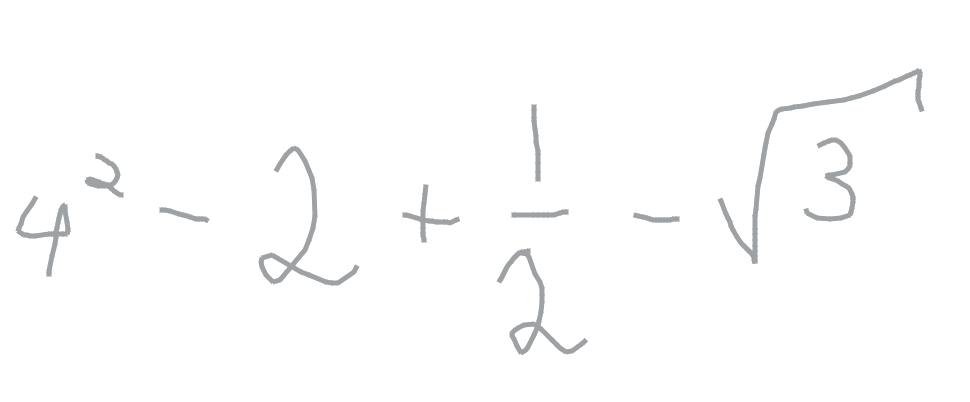
\includegraphics[scale=0.2]{Assets/Chapter3_Method/expression.png}
\end{center}
\centering
    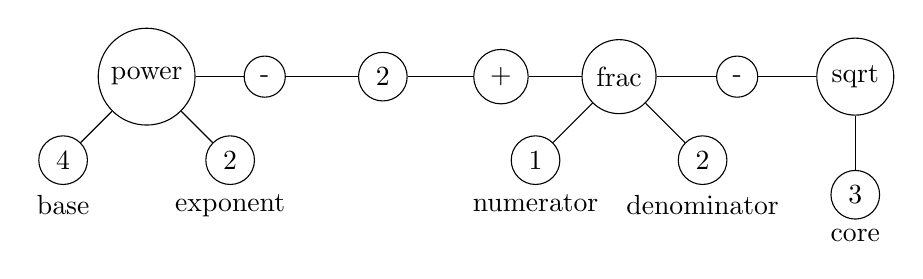
\begin{tikzpicture}[-,',auto,node distance=1.5cm,main node/.style={circle,draw}]
    \node[main node] (2) {power};
    \node[main node] (3) [right of=2] {-};
    \node[main node] (4) [right of=3] {2};
    \node[main node] (5) [right of=4] {+};
    \node[main node] (6) [right of=5] {frac};
    \node[main node] (7) [right of=6] {-};
    \node[main node] (8) [right of=7] {sqrt};
    
    \node[main node] (9) [below left of=2, label=below:base] {4};
    \node[main node] (10) [below right of=2, label=below:exponent] {2};
    
    \node[main node] (11) [below left of=6, label=below:numerator] {1};
    \node[main node] (12) [below right of=6, label=below:denominator] {2};
    
    \node[main node] (13) [below of=8, label=below:core] {3};

    \path[every node/.style={font=\sffamily\small}]
        (2) edge node [right] {} (3)
        (3) edge node [right] {} (4)
        (4) edge node [right] {} (5)
        (5) edge node [right] {} (6)
        (6) edge node [right] {} (7)
        (7) edge node [right] {} (8)
        (2) edge node [right] {} (9)
        (2) edge node [right] {} (10)
        (6) edge node [right] {} (11)
        (6) edge node [right] {} (12)
        (8) edge node [right] {} (13);

    \end{tikzpicture}
    \caption{An input expression and the resulting context tree.}

\label{fig:interpretation-tree1}
\end{figure}

The system understands several mathematical notation elements, including square roots, fractions and exponents. Each of these elements has their own set of grammatical or positional rules that are used to find them (explained in section \ref{interpretation-square-roots} - \ref{interpretation-exponents}). In addition to these elements, some special symbols such as the equal sign and the multiplication dot are found and classified in this step (see section \ref{interpretation-special-symbols}).

\subsubsection{The main function}
The main function in the interpretation system orchestrates the order of what element to search for. The order of elements searched for is:

\begin{enumerate}
    \setlength\itemsep{0.3em}
    \item Square roots
    \item Fractions
    \item Equal signs
    \item Multiplication dots
    \item Power groups, base and exponent
\end{enumerate}

The recursive part of this algorithm occur through the square roots, fraction and exponents. If the body of a square root contains more than one symbol or object, the whole group is sent recursively back to the main function. The same applies for the numerator and denominator found in fractions and for exponent-groups. The reason for this is to further search for context in these subgroups. For instance, fractions can have fractions as their numerator and exponents can consist of smaller expressions. 

This search process can be illustrated by a flowchart:

\begin{figure}[H]
\centering
    \begin{tikzpicture}[->,',auto,node distance=1.5cm,main node/.style={circle,draw},sub node/.style={draw}]
    \node[main node] (1) [label=above:Input] {};
    \node[sub node] (2) [below of=1] {Sqrt};
    \node[sub node] (3) [below of=2] {Frac};
    \node[sub node] (4) [below of=3] {$=$};
    \node[sub node] (5) [below of=4] {$\cdot$};
    \node[sub node] (6) [below of=5] {power};
    \node[main node] (7) [below of=6,label=below:Output] {};

    \path[every node/.style={font=\sffamily\small}]
        (1) edge node [right] {} (2)
        (2) edge node [right] {} (3)
        (3) edge node [right] {} (4)
        (4) edge node [right] {} (5)
        (5) edge node [right] {} (6)
        (6) edge node [right] {} (7)
        
        (2) edge[bend right=80] node [left] {core} (1)
        (3) edge[bend left=90] node [left] {numerator/denominator} (1)
        (6) edge[bend right=90] node [left] {exponent} (1);

    \end{tikzpicture}
    \caption{Flowchart of the order and recursion.}

\label{fig:interpretation_flowchart}
\end{figure}

To find the contents of a body (numerators, denominators, square roots), the interpretation system uses the positional values of the input symbols to check whether they are inside the bounds of an area or not. If their middle point is inside this area, they are added to the output group of the area search. This area is limited by a set of maximum and minimum x- and y-coordinates. These limits comes from a set of parameters required by the main function and the positional values of control units (square roots, fraction bars).

If a square root-, fraction- or exponent-element is found, the system creates an object of the correct type and links the relevant symbols to it. When creating one of these objects the traces for each of the input symbols are combined and new positional and proportional attributes are found.

Details about how these elements are found are described in the next sections.

\subsubsection{Square roots}
\label{interpretation-square-roots}

The symbols classified as square roots are first inserted into a new list and sorted by width, to make sure that the recursive logic is maintained. The widest one is most likely the outermost one if there are roots within roots, and is evaluated first. To find a square root body the system searches for objects within the bounds specified by the positional attributes of the square root. In addition to using the attributes described in section \ref{preprocessing_and_segmentation}, the square roots also uses the x-value of the lowest point, which is the bottom left corner in the image below.

\begin{figure}[H]
\centering
    \begin{tikzpicture}
        \node[anchor=south west,inner sep=0, scale=0.5] at (0,0) {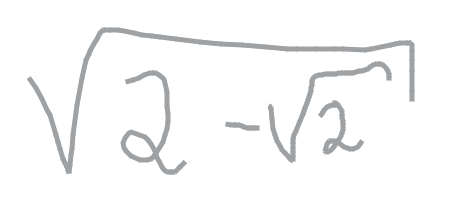
\includegraphics[width=\textwidth]{Assets/Chapter3_Method/interpretation-sqrt.png}};
        \draw[red, thick] (1.2,0.6) rectangle (6.7,2.8);
        \draw[blue, thick] (4.7,0.8) rectangle (6.3,2.3);
    \end{tikzpicture}
    \label{fig:interpretation}
\caption{Search area of square roots.}
\end{figure}

All the symbols and objects found inside are linked to the square root object as the body. This body is then sent recursively through the main function to find the context within the square root.

\begin{figure}[H]
\begin{center}
    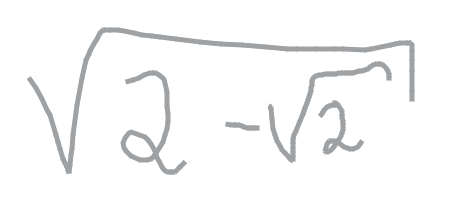
\includegraphics[scale=0.5]{Assets/Chapter3_Method/interpretation-sqrt.png}
\end{center}
\centering
    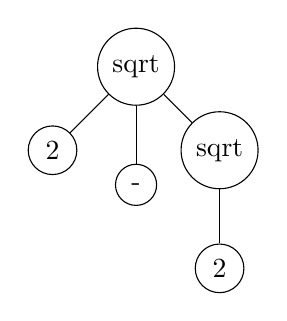
\begin{tikzpicture}[-,',auto,node distance=1.5cm,main node/.style={circle,draw}]
    \node[main node] (1) {sqrt};
    \node[main node] (2) [below left of=1] {2};
    \node[main node] (3) [below of=1] {-};
    \node[main node] (4) [below right of=1] {sqrt};
    \node[main node] (5) [below of=4] {2};

    \path[every node/.style={font=\sffamily\small}]
        (1) edge node [right] {} (2)
        (1) edge node [right] {} (3)
        (1) edge node [right] {} (4)
        (4) edge node [right] {} (5);

    \end{tikzpicture}
    \caption{An expression with a square root inside a square root and the resulting context tree.}

\label{fig:segmentation}
\end{figure}

\subsubsection{Fractions}

To find fractions the system searches for fraction bars by running the input symbols classified as minus signs through a test. To be classified as a fraction bar a minus sign must comply with one of the following cases:

\begin{itemize}
    \setlength\itemsep{0em}
    \item Have at least one symbol in the area over and under itself.
    \item Have at least two symbols in either the area over or the area under itself.
    \item Be the only minus sign in the input list and have at least one symbol in the area over or under itself.
\end{itemize}

To find the numerator and denominator of a fraction, the system searches for symbols in the area over and under the minus signs. The width of this area is specified by the leftmost and rightmost coordinate of the minus sign, and the height is limited only if the area is between two fraction bars (the area that searches for the number 3 in the image below). The denominators and numerators found are also sent recursively through the main function to further look for context.

\begin{figure}[H]
\centering
\begin{tikzpicture}[-,',auto,node distance=1.5cm,main node/.style={circle,draw}]
    \node[anchor=south west,inner sep=0] (image) at (0,0) {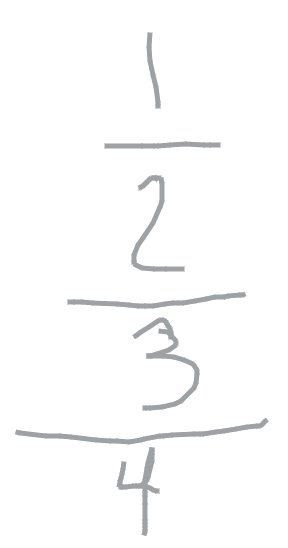
\includegraphics[width=0.2\textwidth]{Assets/Chapter3_Method/interpretation-frac.png}};
    
    \draw[red, thick] (0.2,0) rectangle (2.7,1.1);
    \draw[red, thick] (0.2,1.3) rectangle (2.7,6);
    \draw[blue, thick] (0.7,1.2) rectangle (2.5,2.5);
    \draw[blue, thick] (0.7,2.6) rectangle (2.5,6);
    \draw[purple, thick] (1.1,2.55) rectangle (2.2,4.1);
    \draw[purple, thick] (1.1,4.15) rectangle (2.2,6);
    
    \node [main node] (1) [right of=image, xshift=4cm, yshift=2cm]{frac};
    \node [main node] (2) [below left of=1]{frac};
    \node [main node] (3) [below right of=1]{4};
    \node [main node] (4) [below left of=2]{frac};
    \node [main node] (5) [below right of=2]{3};
    \node [main node] (6) [below left of=4]{1};
    \node [main node] (7) [below right of=4]{2};
    
    \node[rotate=45] (8) [below right of=5, xshift=-1cm, yshift=0.3cm]{denominators};
    \node[rotate=45] (9) [left of=2, xshift=0.5cm, yshift=1cm]{numerators};
    
    \path[every node/.style={font=\sffamily\small}]
        (1) edge node [right] {} (2)
        (1) edge node [right] {} (3)
        (2) edge node [right] {} (4)
        (2) edge node [right] {} (5)
        (4) edge node [right] {} (6)
        (4) edge node [right] {} (7);
\end{tikzpicture}
\caption{The search areas of a fraction expression with recursion and the corresponding context tree. The widest minus sign is considered the root fraction.}
\end{figure}

\subsubsection{Exponents}
\label{interpretation-exponents}

Exponents are found by checking if a pair of following symbols or objects forms a power-group. A power group is the object used for base/exponent groups. To form one of these groups the exponent has to be positioned such that the following rules are complied with:
\begin{itemize}
    \setlength\itemsep{0em}
    \item The lowest point of the exponent has to be higher up than the middle y-value of the base.
    \item The middle y value of the exponent has to higher up than the upper fourth of the base.
\end{itemize}
In addition, there is a special case rule if the exponent is an operator (-, +). Then, the lowest point of the exponent has to be higher up than the upper fourth of the base. The purpose of this is to increase the threshold to let a minus sign be the beginning of an exponent. Without this rule, expressions like '$2-2$' might mistakenly be recognized as '$2^{-}2$', since a minus sign is flat, and can easily be interpreted as an exponent based on the rules above.

\begin{figure}[H]
\centering
\begin{tikzpicture}[-,',auto,node distance=1.5cm,main node/.style={circle,draw}]
    \node[anchor=south west,inner sep=0] (image) at (0,0) {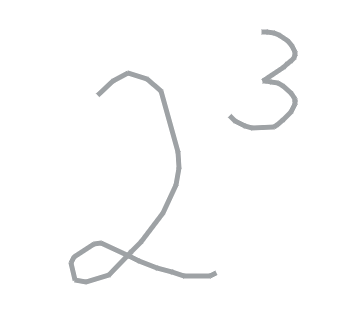
\includegraphics[width=0.2\textwidth]{Assets/Chapter3_Method/interpretation-exp.png}};
    \node[anchor=south west,inner sep=0] (image2) [left of=image, xshift=6cm] {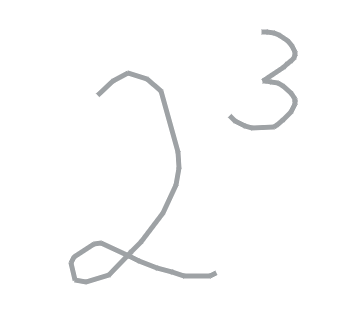
\includegraphics[width=0.2\textwidth]{Assets/Chapter3_Method/interpretation-exp.png}};
    
    \draw[-, red] (0,1.3) -- node[left, xshift=-2cm, yshift=-0.1cm] {middle point of base} (4,1.3);
    \draw[-, red] (0,1.65) -- node[left, xshift=-2cm, yshift=0.1cm] {lowest point of exp} (4,1.65);
    \draw[-, blue] (5,2.05) -- node[right, xshift=1.5cm, yshift=0.1cm] {middle point of exp} (8,2.05);
    \draw[-, blue] (5,1.7) -- node[right, xshift=1.5cm, yshift=-0.1cm] {top fourth of base} (8,1.7);
\end{tikzpicture}
\caption{Example of a power group and visualization of the first and second rule.}
\end{figure}

The system also supports groups of symbols and objects as base or exponent. Exponents within exponents are also supported. When a base and exponent are found, the system continues to check if the next symbol also is an exponent for the same base. This search continues until a symbol conflicts with one of the rules. All the found symbols are then sent recursively through the main function again.

\begin{figure}[H]
    \centering
    \begin{tikzpicture}[-,',auto,node distance=1.5cm,main node/.style={circle,draw}]
        \node[anchor=south west,inner sep=0] (image) at (0,0) {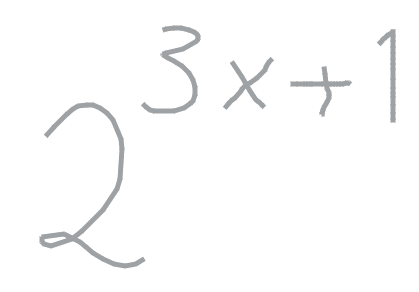
\includegraphics[width=0.2\textwidth]{Assets/Chapter3_Method/interpretation-exp2.png}};
    
        \node[anchor=south west,inner sep=0] (image2) [right of=image, xshift=4cm] {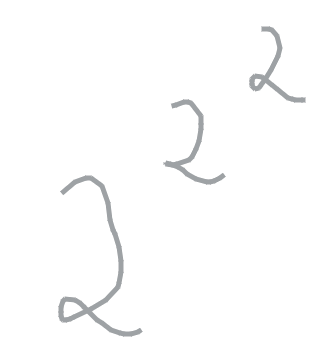
\includegraphics[width=0.2\textwidth]{Assets/Chapter3_Method/interpretation-exp3.png}};
        
        \node [main node] (1) [below of=image, yshift=-1.5cm]{power};
        \node [main node] (2) [below left of=1]{2};
        \node [main node] (3) [below right of=1]{group};
        \node [main node] (4) [below left of=3]{3};
        \node [main node] (5) [below of=3, xshift=-0.4cm]{x};
        \node [main node] (6) [below of=3, xshift=0.4cm]{+};
        \node [main node] (7) [below right of=3]{1};
        
        \node[rotate=0] (13) [left of=1, xshift=-0.2cm, yshift=-0.4cm]{Base};
        \node[rotate=0] (14) [right of=1, xshift=1cm, yshift=-0.4cm]{Exponent};
        
        \node [main node] (8) [below of=image2, yshift=-1.5cm]{power};
        \node [main node] (9) [below left of=8]{2};
        \node [main node] (10) [below right of=8]{power};
        \node [main node] (11) [below left of=10]{2};
        \node [main node] (12) [below right of=10]{2};
        
        \node[rotate=0] (15) [left of=11, xshift=0.5cm, yshift=0.4cm]{Bases};
        \node [] (16) [right of=10, xshift=0.4cm, yshift=-0.2cm]{Exponents};

        \path[every node/.style={font=\sffamily\small}]
            (1) edge node [right] {} (2)
            (1) edge node [right] {} (3)
            (3) edge node [right] {} (4)
            (3) edge node [right] {} (5)
            (3) edge node [right] {} (6)
            (3) edge node [right] {} (7)
            (8) edge node [right] {} (9)
            (8) edge node [right] {} (10)
            (10) edge node [right] {} (11)
            (10) edge node [right] {} (12);
            
    \end{tikzpicture}
    \caption{Power groups and their corresponding context tree.}
\end{figure}


\subsubsection{Special case symbols}
\label{interpretation-special-symbols}

In this system there are two special case symbols: the equal sign and the multiplication dot operator. These require special treatment due to how the segmentation and classification steps are designed. An equal sign usually consist of two traces which would be interpreted as two minus signs since the segmentation step splits them up. The multiplication sign is a small dot that, when preprocessed and scaled up, would look similar to other round symbols like 0 and $\theta$. It would therefore most likely be misclassified.

To find equal signs the system searches for minus signs that are of similar size and lined up like an equal sign. To do this, each possible pair of minus signs in the input list are tested against some rules. The pair is classified as an equal sign only if these points are fulfilled:

\begin{itemize}
    \setlength\itemsep{0em}
    \item The width of the minus signs has to be similar. The difference in width has to be less than their average width.
    \item The difference between the centre x-coordinate value has to be less than a third of their combined width.
    \item The difference between the centre y-coordinate value has to be less than a their average width.
\end{itemize}

These rules became such after many rounds of testing. The idea behind them was to be as general as possible.

To find the multiplication signs small symbols are searched for by looking at width, height and area. Symbols are classified as multiplication signs if their area, height and width are within a small threshold. In addition, the height and width has to be similar, one of them can't be more than twice the length of the other one.


\subsection{Converting to \LaTeX}
After the context has been found, the results can be converted to the corresponding \LaTeX -code. For this, the truth values to all the output objects are combined in a string by a function. This function also has to be recursive, since the output objects might be fractions, square root or base-exponent groups. If a fraction is found, the contents of the numerator and denominator are sent through the same function. The same applies for the square root cores, exponents and bases.

\section{The project process} % 
The project process in terms of software engineering methodology has been a mix between multiple concepts and paradigms. Modern Agile was used in this project, it emphasizes four basic principles that made our project flow optimal. The four principles are make people awesome, deliver value continuously, make safety a prerequisite and experiment and learn rapidly. \cite{agile_modern_????}


\section{Teamwork and roles} %
Every project participant had roles as a full stack software engineer and research engineer. Initially the resources were distributed between three domains, front end, back end and machine learning research. No clear structure was enforced and the roles were unconstrained, because it was thought that different mindsets could improve quality and productivity. The distribution of roles and tasks were based on the sprint goals.
